\setcounter{figure}{0}
\setcounter{table}{0}
\section{ECG监测与记录应用的设计与实现}
\subsection{应用程序需求分析}
通过分析ECG波形的基本形态、关键特征并参考已有设计的特点后,能够归纳出用户对ECG监测与记录应用的需求。

\subsubsection{ECG信号的产生与特点}

心脏通过心肌组织的受控收缩/舒张完成泵血的工作,而心肌组织由心肌细胞组成。每个心肌细胞含有钾、纳、钙等离子,通过输入和泵出这些离子,心肌细胞完成舒张和收缩的过程,相应的,由这些过程造成的细胞内外电位差变化被称为”复极”和”除极”\cite{moreno_android_2012}。而通过在人体表面施加电极(被称为导联),记录下这种电位差变化而形成的图形被称为心电图(Electrocardiogram,ECG)\cite{_zhenduanxue_2013}。如图\ref{fig3-1}所示,除极过程和复极过程表现出来的细胞内外电势差方向是相反的,因此两过程形成的波形方向也相反,心电图也因此包含正负两个方向的电位变化。

\begin{figure}[htb]
\begin{center}
\begin{minipage}[b]{0.55\linewidth}
\begin{center}
  \subfigure[]{
  \begin{minipage}[b]{\textwidth}
  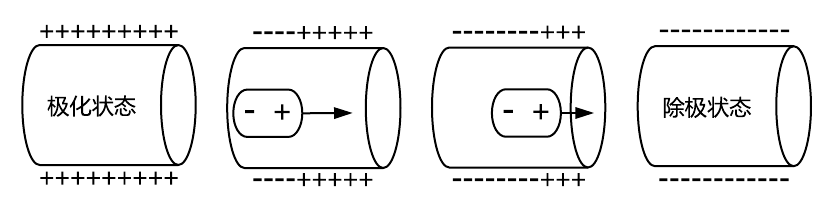
\includegraphics[width=\textwidth]{fig3-1a.png}
  
  \end{minipage}
  }
  \subfigure[]{
  \begin{minipage}[b]{\textwidth}
  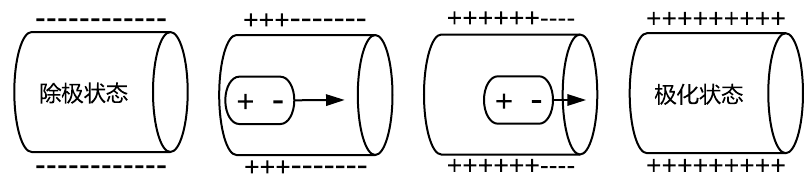
\includegraphics[width=\textwidth]{fig3-1b.png}
  \end{minipage}
  }
\end{center}
\end{minipage}
~~~~
\begin{minipage}[b]{0.4\linewidth}
  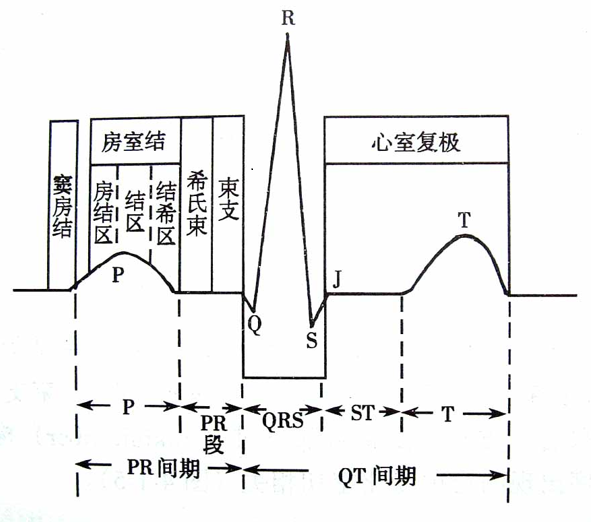
\includegraphics[width=0.9\textwidth]{fig3-2.png}  
\end{minipage}\\[-10pt]
\begin{minipage}[t]{0.55\linewidth}
\caption{\label{fig3-1}心肌细胞的除极与复极过程:(a)为除极过程,(b)为复极过程}
\end{minipage}
\begin{minipage}[t]{0.4\linewidth}
\caption{\label{fig3-2}ECG信号波形示意图}
\end{minipage}
\end{center}
\end{figure}

若将所有心肌细胞内外电势差看为一个电矢量,则它的位移局限在心肌内,可近似看作电偶固定在心脏中心,心脏中不同部位的心肌组织除极时间存在差异,从而造成了这个矢量方向的转动。同时,电矢量的强度也随心肌大小、薄厚的改变而改变。因此将导联放置在身体不同位置时,对应的电矢量变化不同,测得的心电图也不同。实际的心电图测量往往包含肢导联和胸导联,不同的导联放置位置不同。在临床实践中通常综合12个导联的ECG波形来判断心脏状态。

单个导联的心电图通常包含P波、QRS波群和T波,这是根据波的大小和形态而划分的(见图\ref{fig3-2})。通过观察一幅ECG图像的PQRST波及其特点,能够了解心脏某部分或整体的搏动状况。在医学生的训练中,以下ECG图像特征的观察备受强调:

\begin{itemize}
\item 两个P波或R波的间隔时间(PP间期或RR间期);
\item PP或RR间期的离散程度;
\item P波持续时间;
\item P波振幅;
\item P波与R波的间隔时间(PR间期);
\item QRS波群的间隔时间(QRS间期);
\item S波结束与T波开始之间的间隔时间;
\item 经过矫正的QT间期(即$\mathrm{QT_c}$,可通过$\mathrm{QT_c = \frac{QT}{\sqrt{RR}}}$计算,其中QT表示实际QT间期,RR表示RR间期)
\end{itemize}

除此以外,还有一些基于波形形态的观测(如QRS波的主波方向)在诊断中也十分重要。这些波形形态能够反映心脏房室肥大情况、心肌缺血情况、心肌是否坏死等。

通过了解ECG信号的产生原理和主要特征,医护人员对于ECG监测记录应用的需求便可以总结出来。

\subsubsection{用户需求}
用户的需求直接决定了功能的设计和实现。本研究假定使用ECG监测记录应用的用户群体为医护人员,根据ECG信号的基本特征,可以将用户的需求总结如下:

\textbf{业务需求:}能够实时观察ECG波形的变化;能够快速了解到波形中某些时刻的幅值;能够观察多个周期ECG的波形以观察其形态;能够观察ECG波形中较为具体的细节。

\textbf{功能需求:}能够记录测量到的ECG波形;能够提取关键的ECG信号特征(如心率)并展示出来;能够提供测量ECG波形中两点间的时间间隔和幅值差;能够计算出某些特征值的波动情况(如心率的波动情况)。

\textbf{非功能性需求:}应用运行时应顺畅无卡顿;波形记录应能准确记录某时间点对应的数值;界面应该易于使用,没有误导性;应用的核心功能应该提供接口,以便二次开发。

根据上述业务及功能需求,总结出该应用的UML用例图如下:

\begin{figure}[htbp]
\centering
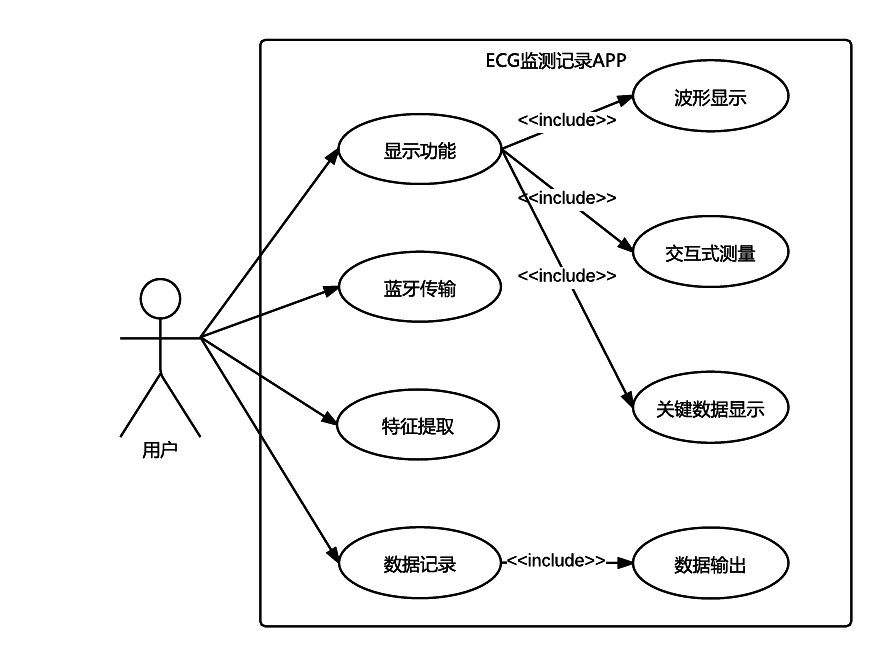
\includegraphics[width=0.8\columnwidth]{fig3-3.png}
\caption{
\label{fig3-3}
ECG监测记录应用的UML用例图
}
\end{figure}

\subsection{系统结构设计}

以应用的功能为参考,本研究使用模块化结构实现应用的功能,保证每个类对相应对象的抽象更加准确。根据上文总结的各类需求,将应用的设计与实现分为蓝牙传输模块、显示模块、数据库管理模块和数据分析模块四个部分,各个模块之间呈现松耦合的关系,通过在主线程中接受各模块信息、调用各模块的成员函数实现应用的功能。

\subsection{各模块的设计与实现}
\subsubsection{显示模块的设计与实现}
显示模块在保证波形顺畅显示的同时,也需要满足用户观察波形的需求和交互式测量的需求。如1.2.2节所述,现有研究的显示方式无法解决用户操作和波形完全显示之间的矛盾。为解决此问题,本研究在设计显示模块时利用了横竖屏各自的特点,设计了两种波形显示方式:竖屏时概略显示波形,同时提供更多的操作选项;横屏时着重显示波形及其细节,辅以显示波形的关键特征。两种界面的示意图如下所示:

\begin{figure}[htb]
  \centering
  \subfigure[应用竖屏主页面]{
    \label{fig3-4a} %% label for first subfigure
    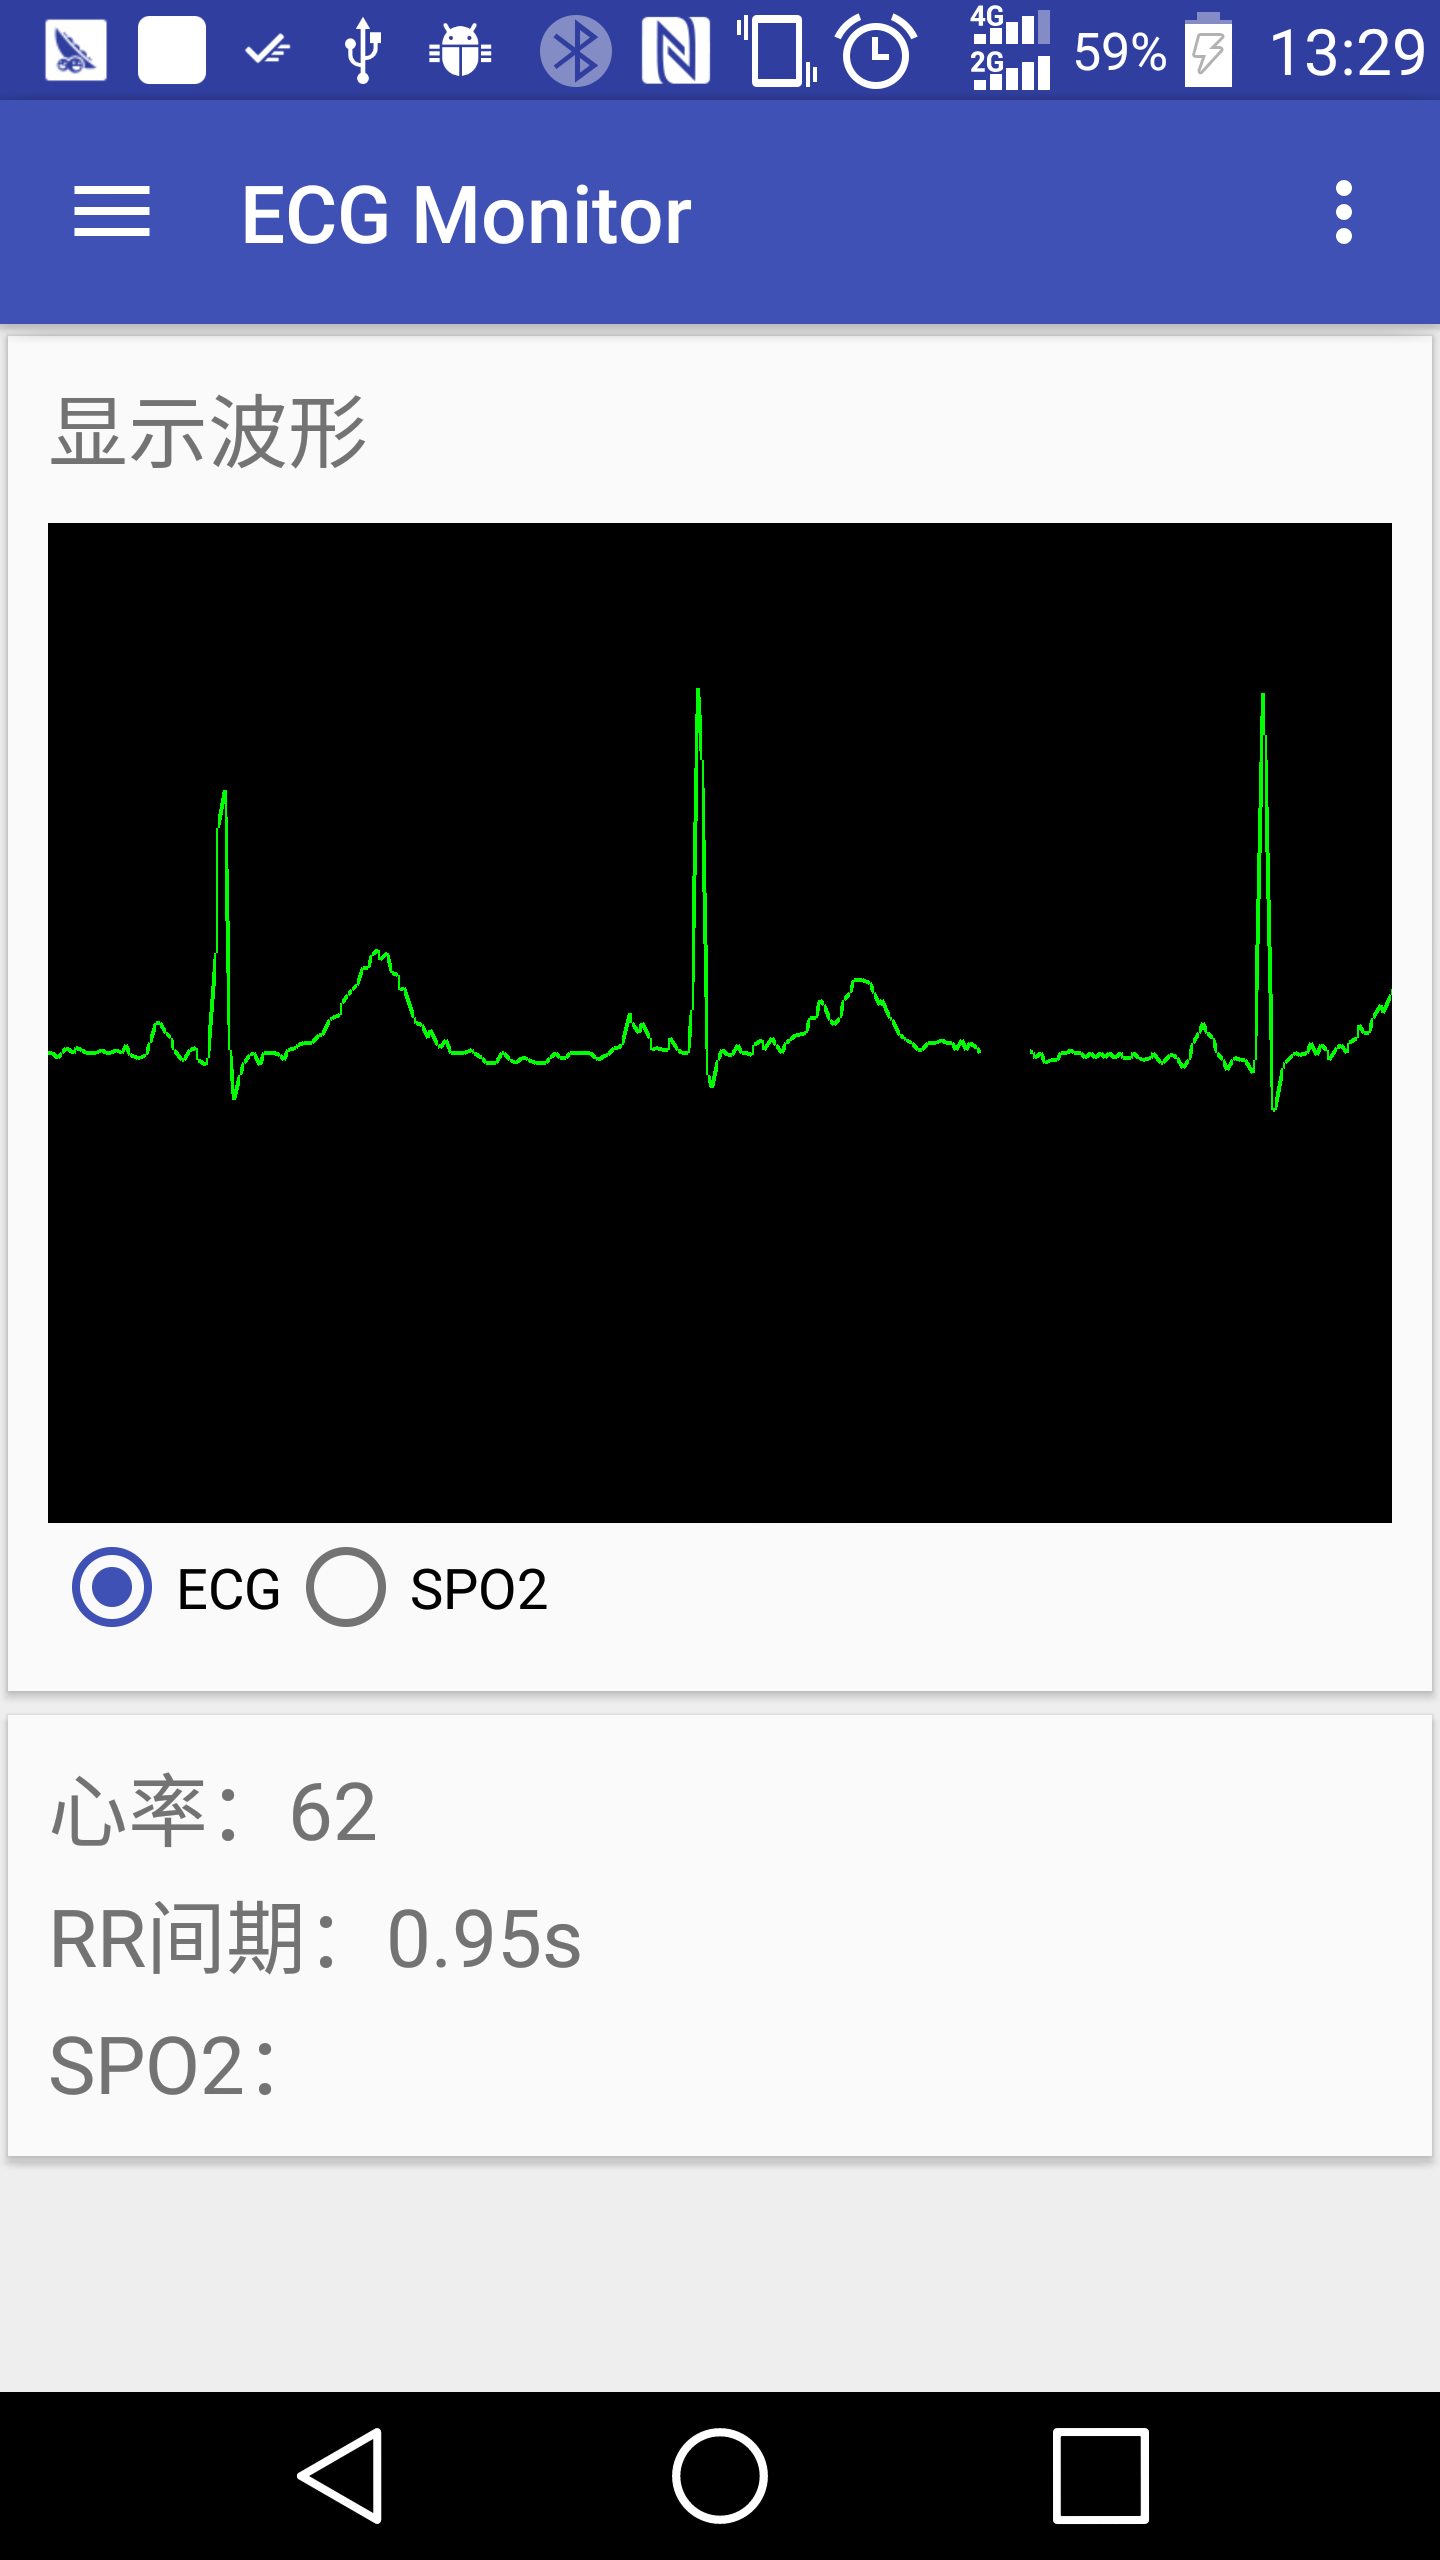
\includegraphics[width=0.35\textwidth]{fig3-4.png}}
  \hspace{0.5cm}
  \subfigure[应用竖屏菜单]{
    \label{fig3-4b} %% label for second subfigure
    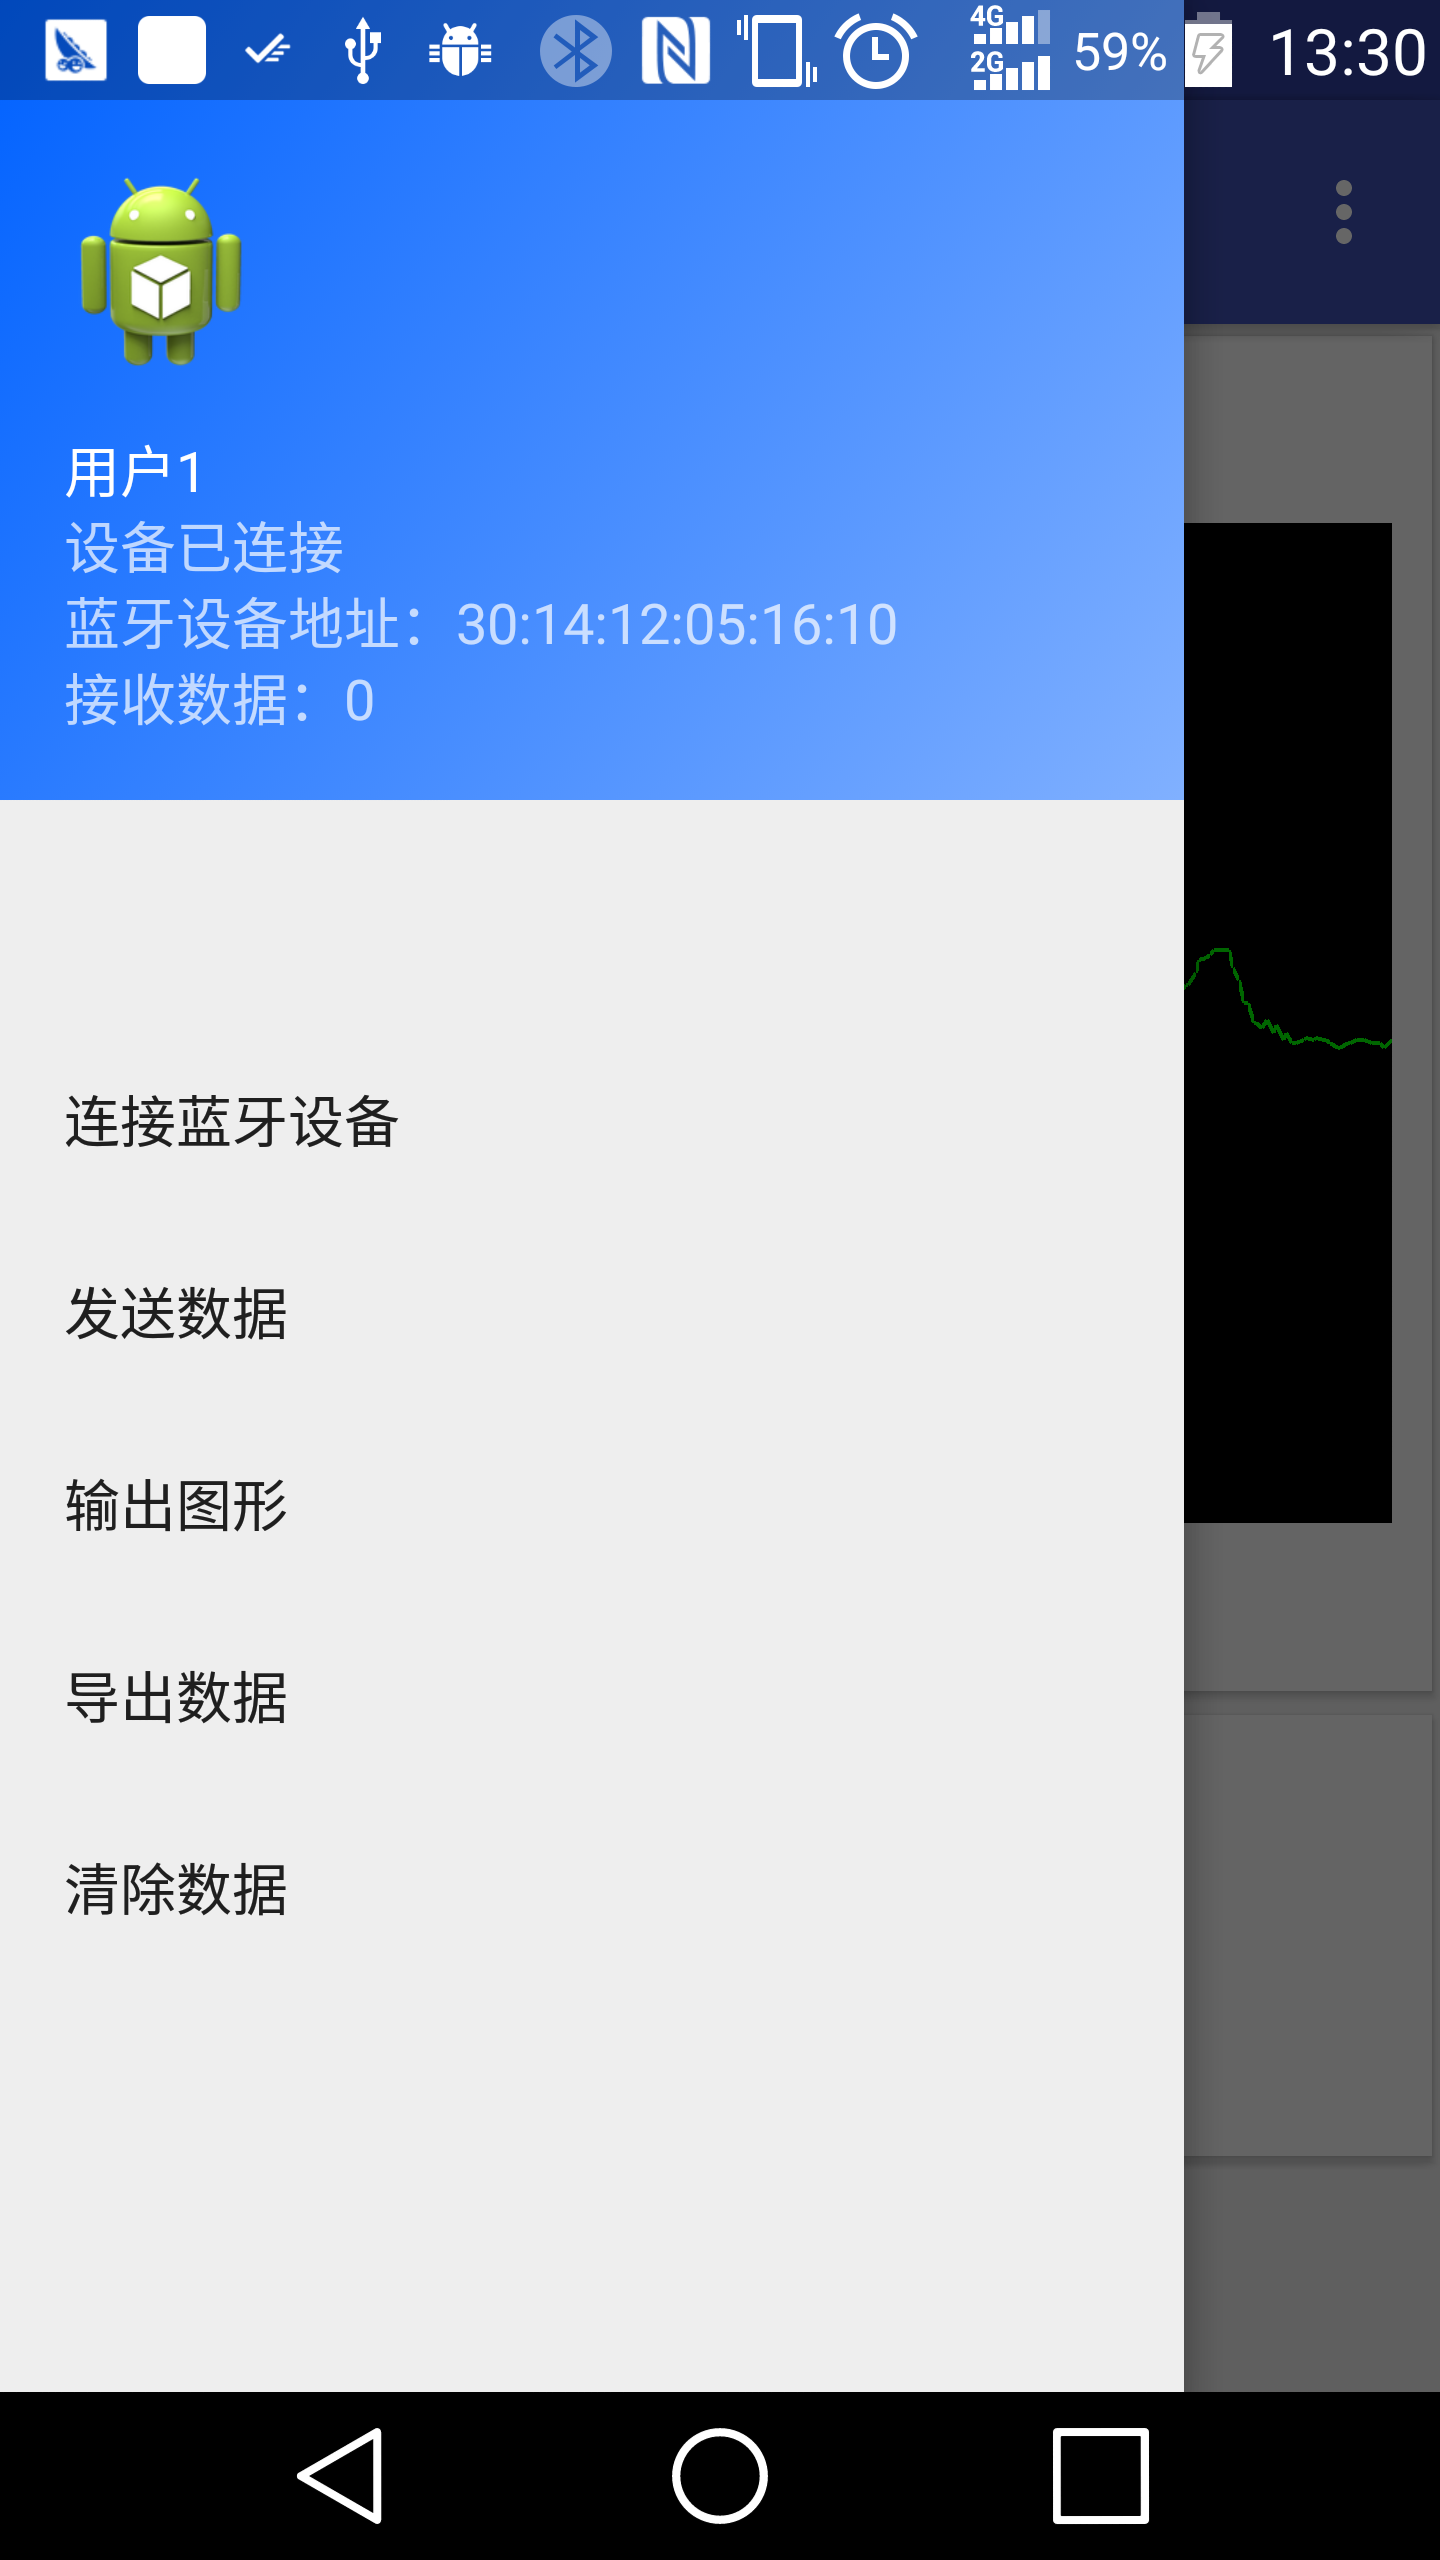
\includegraphics[width=0.35\textwidth]{fig3-5.png}}
  \\
  \subfigure[应用横屏显示]{
    \label{fig3-4c} %% label for second subfigure
    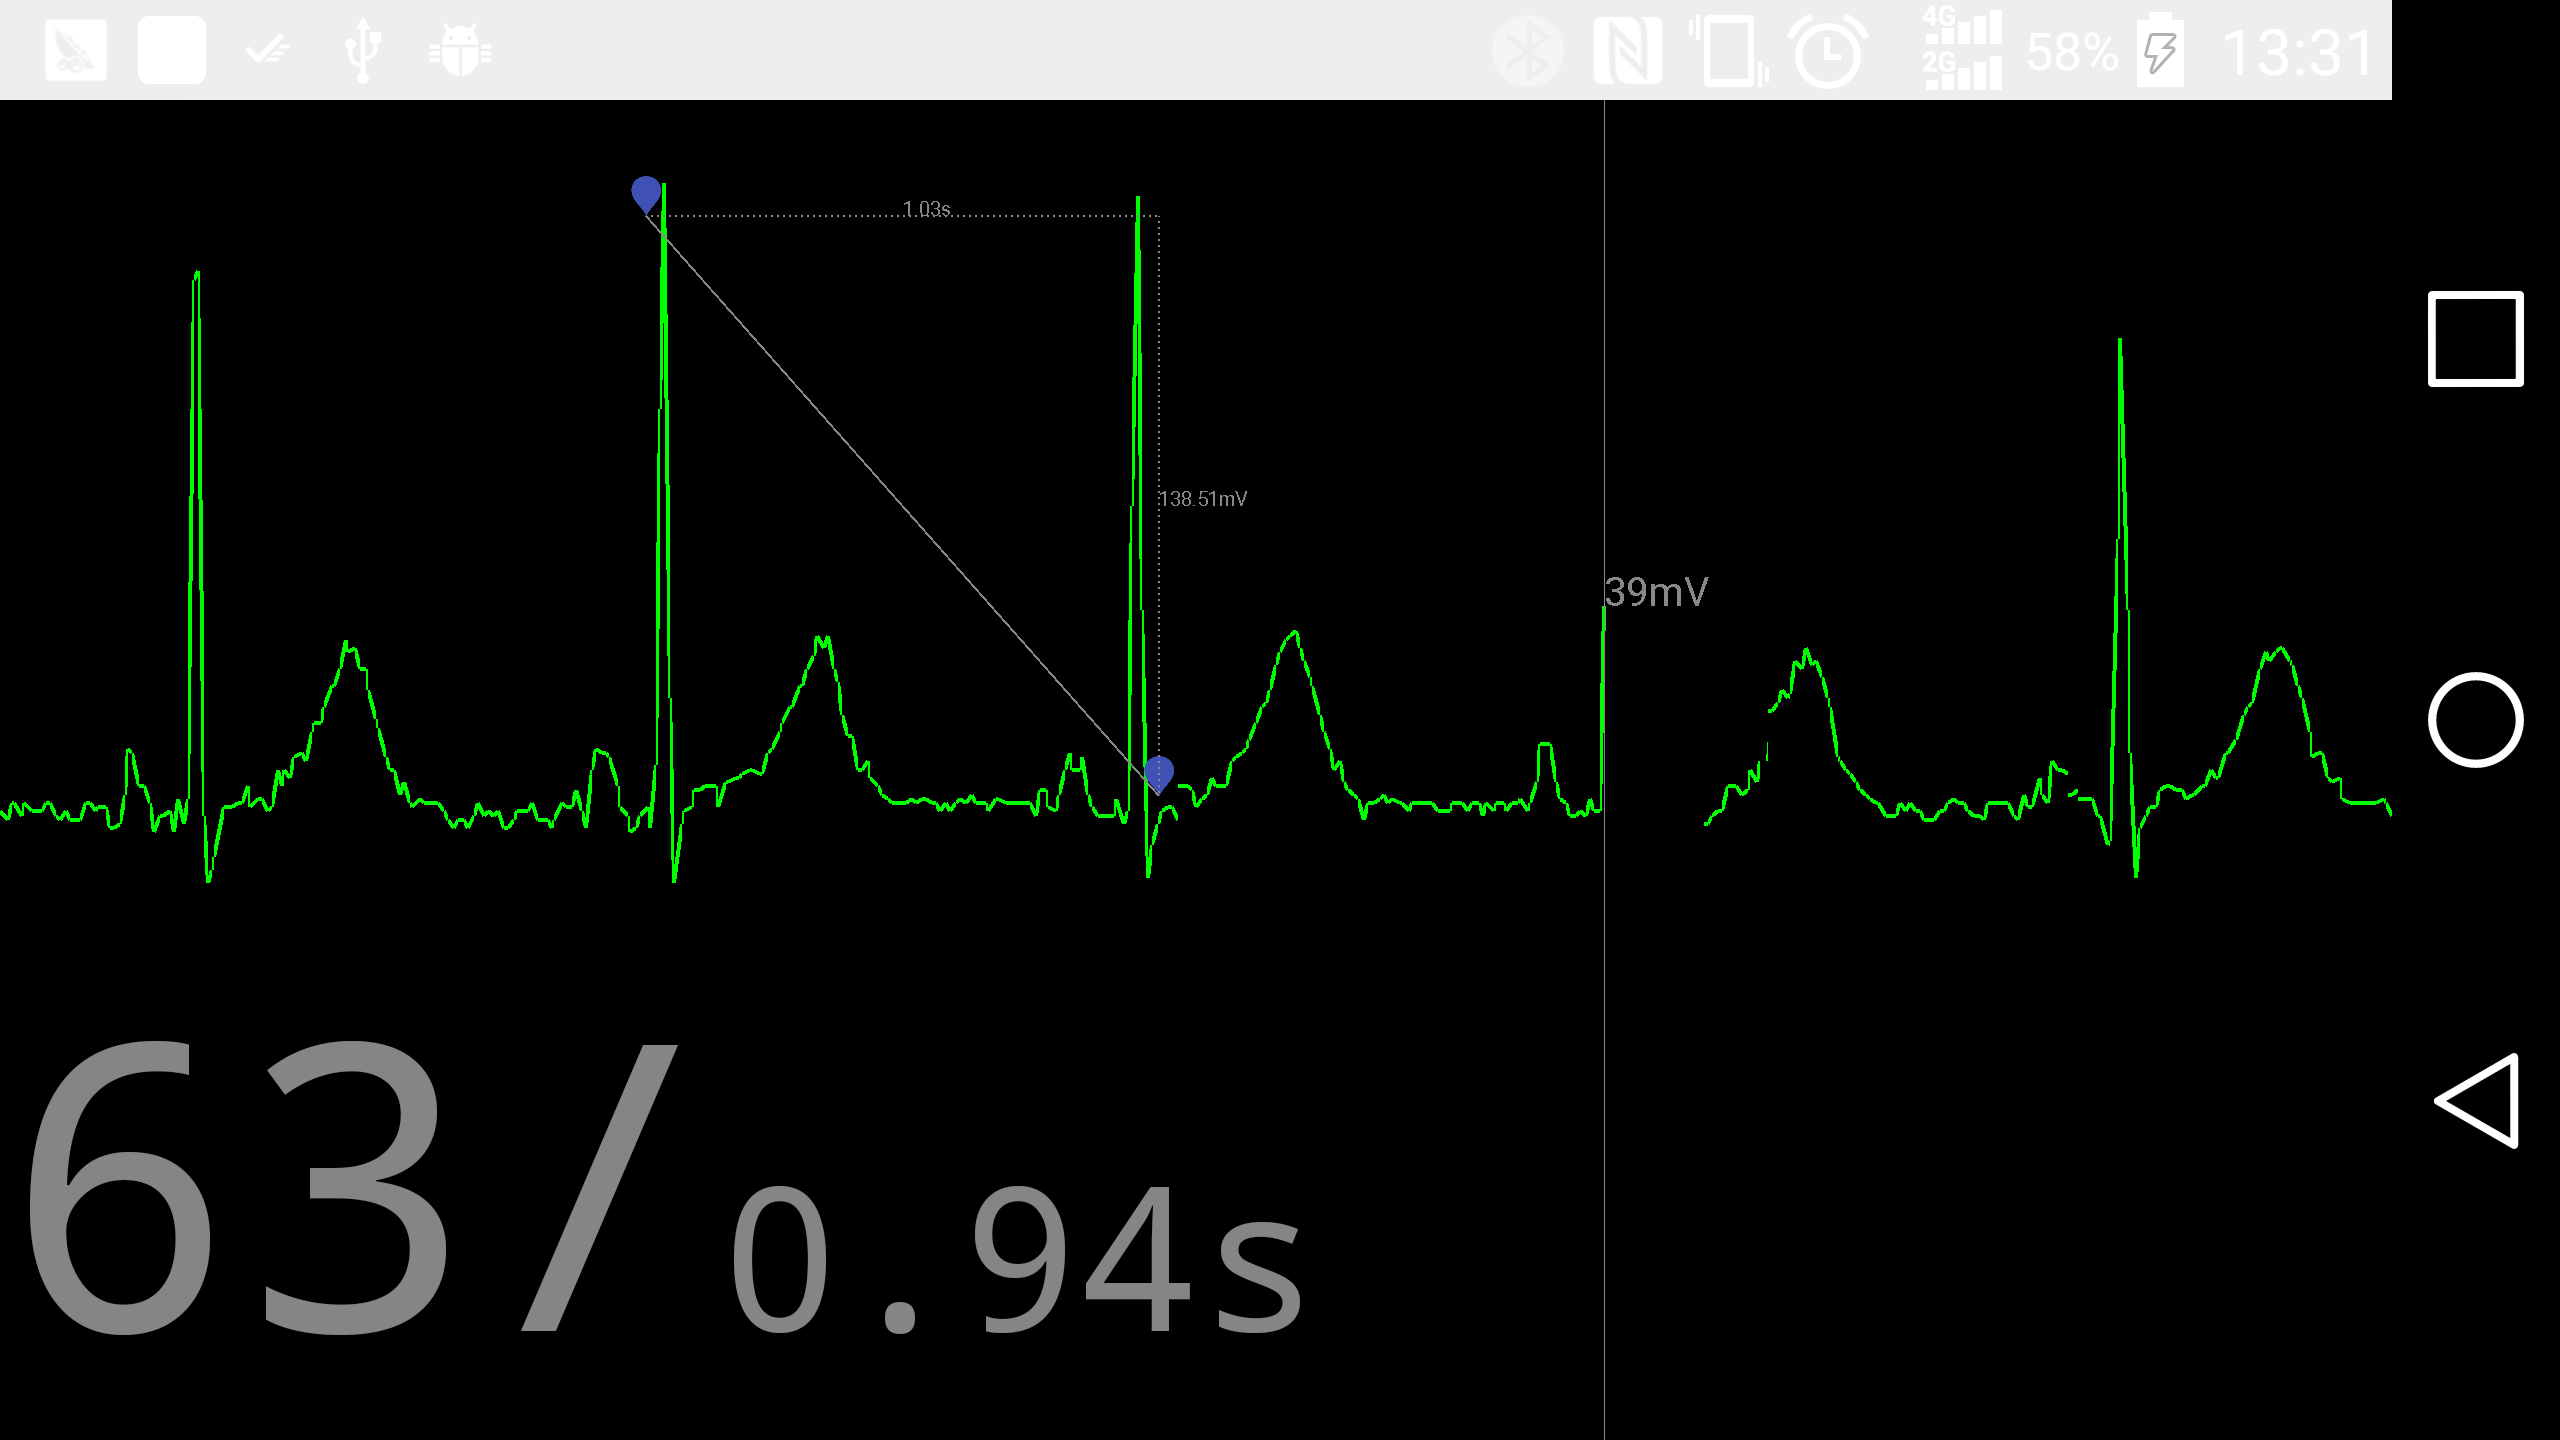
\includegraphics[width=0.7\textwidth]{fig3-6.png}}
    \caption{应用的布局方式}
  \label{fig3-456} %% label for entire figure
\end{figure}

在Android平台中实现横竖屏布局切换较为容易:在工程的res资源文件夹中准备两种布局文件activity\_main.xml与activity\_main\_land.xml;当屏幕状态改变时,系统会自动调用onConfigurationChanged()方法。通过重写该方法使系统根据不同的屏幕状态选择布局文件和适合屏幕的SurfaceView类。

对于波形的显示,创建DrawSurfaceView类用于管理和绘制显示波形的SurfaceView类。该类需要实现的功能包括:根据获取到的数据绘制波形、显示波形的特征、提供交互式的波形测量方法。针对每种绘制工作,该类使用一条线程实现。

对于绘制波形,每个数据点在SurfaceView中的坐标是关键。首先,按数据值占ECG信号最大值的比例计算出该数据点在显示框中的纵坐标;对于横坐标,以数据点的序号作为绘制的横坐标,当横坐标超出绘制区宽度则从头绘制。确定坐标以后启动绘制进程,锁定画布,根据屏幕方向更新对应的SurfaceView即可。但由于Android系统存在其他后台活动的原因,当ECG信号发送频率达到300Hz以上时波形显示将会出现严重的丢帧现象。虽然ECG采集速率一般低于300Hz,但ECG传感器发送频率可能高于此值。因此在绘制波形时对收到的信号以20Hz重新采样,得到流畅的显示效果,同时对波形的观察没有太大影响,此时信号记录按接收速率保存数据,并不重新采样。总体绘制的步骤使用Java代码表示如下:

\begin{center}
\begin{lstlisting}
public DrawSurfaceView() { 
    x = 1; 
    shouldRefresh = false;
    setTimer(50);
} 
...
public void drawPoint(int drawX, int drawY) { 
    if (shouldRefresh) { 
        calculateXandY(x,y);
        shouldRefresh = false; 
        drawThread = new DrawThread(); 
        drawThread.start(); 
    } 
} 
...
private class DrawThread extends Thread{
...
    @Override       
    public void run(){
        try{
            if(x>surfaceWidth) x = 0;
            lockCanvas(lastx,0,x+100,surfaceHeight)
            drawLine(lastX,lastY,x,y);
        }finally{
        unlockCanvasAndPost(canvas);            
        }
    }
}
\end{lstlisting}
\end{center}

对于关键数据(如心率、赋值等),使用drawText()方法绘制在图上即可。对于测量标尺,需要检测onTouch触摸事件以做出响应反馈。对显示标尺的SurfaceView设置onTouchListener监听器,发生触摸时记录该点位置,发生触摸移动时绘制用户画出的直线;结束触摸时显示标尺量出的数据。标尺的绘制同样使用SurfaceView机制,在此不作赘述。标尺的显示效果见图\ref{fig3-456}。

\subsubsection{蓝牙传输模块的设计与实现}

蓝牙传输模块保证了数据的正确接收,当接收到数据后还会向主线程发送信号、提醒主线程即时显示数据、将数据插入数据库。蓝牙传输模块的UML类图如下:

\begin{figure}[htbp]
\centering
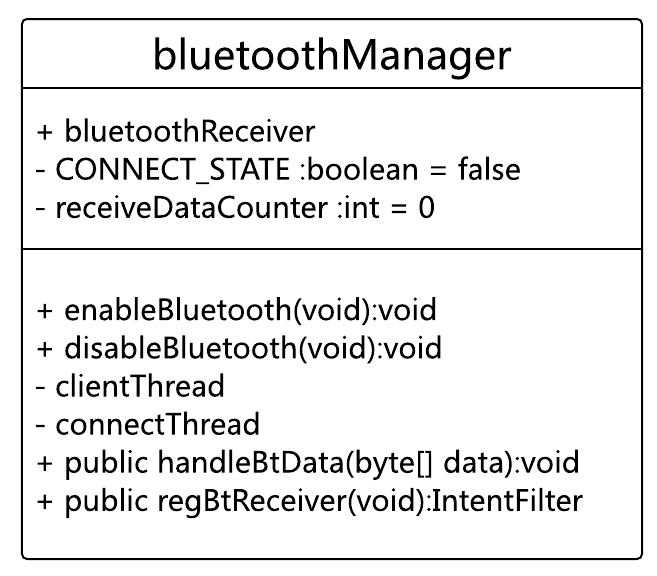
\includegraphics[width=0.5\columnwidth]{fig3-7.png}
\caption{
\label{fig3-7}
蓝牙传输模块的UML类图
}
\end{figure}

其中CONNECT\_STATE负责表明当前连接状态,receiveDataCounter表示接收的数据总数,bluetoothReceiver表明搜索到的蓝牙种类及处理方式。在各项方法中,enableBluetooth()与disableBluetooth()方法负责打开蓝牙、关闭蓝牙;clientThread线程负责建立RFCOMM连接,connectThread负责在已建立的RFCOMM上通过socket循环接收数据,并调用handleBtData()方法处理数据、传送给其他模块;regBtReceiver()方法用来在主线程初始化时注册蓝牙广播接收器。

利用广播接收器(BroadcastReceiver)接收检测到的蓝牙设备是蓝牙连接的开端。在主线程注册蓝牙广播接收器后,若有蓝牙设备探测到,系统发出相应广播,bluetoothReceiver(继承自BroadcastReceiver)被触发,并通过蓝牙设备名称筛选蓝牙设备。当找到需要连接的设备后,获取其地址和设备,开启一个clientThread线程;若bluetoothReceiver收到的是诸如连接断开的异常广播,则采取相应措施。此部分使用Java代码可简单表示如下:
\begin{center}
\begin{lstlisting}
public class bluetoothReceiver extends BroadcastReceiver {
    @Override
    public void onReceive(Context context, Intent intent) {
        String action = intent.getAction();
        String targetName = "hc-bluetooth";
        if (action == ACTION_FOUND) {
            currentDevice = getDevice();
            if (currentDevice.getName() == targetName) {
                CONNECT_STATE = true;
                new clientThread.start();
            }
        } else if (action == ACTION_DISCOVERY_FINISHED) {
            if (!isConnected()) {
                print("搜索结束,没有找到设备");
            }
        } else if (action == ACTION_DISCOVERY_STARTED) {
            print( "搜索开始");
        } else if (action == ACTION_ACL_DISCONNECTED) {
            CONNECT_STATE = false;
            print("连接断开,正在重试连接");
            refreshUI();
        }
    }
}
\end{lstlisting}
\end{center}

在ClientThread线程中,Android手机将使用UUID与蓝牙设备建立一条RFCOMM信道,并且开启connectThread线程。之后,connectThread线程将建立InputStream变量持续接收byte[]类型的数据,直至RFCOMM通道被关闭。由于
\begin{wrapfigure}{l}{15em}%靠文字内容的左侧
\label{fig3-8}
\setlength{\belowcaptionskip}{-20pt}
\setlength{\abovecaptionskip}{0pt}
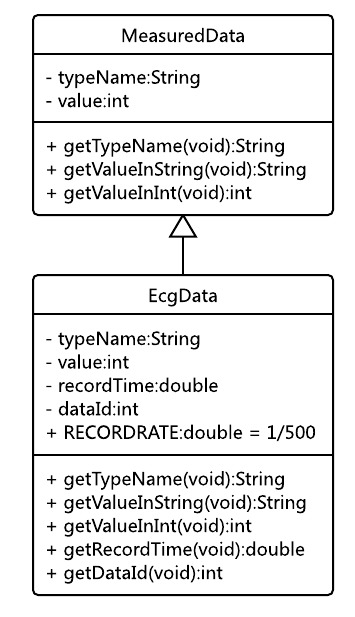
\includegraphics[width=0.4\columnwidth]{fig3-8.png}
\caption{ECG数据类的UML类图}
\end{wrapfigure}
InputStream带有缓存,因此高速传输时数据不会丢失。该线程每接收2byte数据时调用handleBtData处理一次(将数据由byte类型补码形式转化为int类,并插入数据库)。

\subsubsection{数据库管理模块的设计与实现}
为方便各类之间数据传输,所测量数据的格式是经过专门设计的。首先创建MeasuredData类作为所得数据的基类,再创建EcgData类继承MeasuredData,实现ECG数据的存储。两种类的关系如图3-6所示。

其中ECG专用数据结构在其父类的基础上增加了自动建立时间戳、标明数据传输速率的功能。在EcgData的构造函数中,通过数据的序号和传输速率计算出时间戳并赋值给recordTime。若在接收数据时获取系统时间并加盖时间戳,则由于系统后台程序等原因,时间的准确性无法保证。实验证明,以500Hz传输数据时,数据接收缓存中大约会积压50个左右待处理的数据,当之后为这些数据加盖时间戳时,获取的时间已经迟于真正接收它们的时间了(延迟时间约为140ms,足以影响心率的判定)。而使用推算的方式能够保证时间戳的正确。

当一个ECG数据被蓝牙模块接收后,主线程会调用EcgData构造函数创建一个EcgData类的变量并调用EcgDatabaseManager类的成员函数将其插入数据库。该类主要负责数据库的管理和数据的输入输出工作,这些工作均通过对SQLiteDatabase类和SQLiteOpenHelper类的操作实现。当应用程序打开时,该类的构造函数会检查数据库的有效性,并创建或打开数据库ecg.db。相关代码如下:

\begin{center}
\begin{lstlisting}
public HealthDatabaseHelper(Context context) {
    super(context, DATABASE_NAME, null, 1);
}

@Override
public void onCreate(SQLiteDatabase db) {
    db.execSQL("CREATE TABLE IF NOT EXISTS ecg" + "(_id INTEGER PRIMARY KEY " + "AUTOINCREMENT, value INTEGER, time REAL)");
    //empty the ecg table
    db.execSQL("DELETE FROM ecg");
}

@Override
public void onOpen(SQLiteDatabase db) {
    super.onOpen(db);
}
...
ecgDatabase = healthDatabaseHelper.getWritableDatabase();
\end{lstlisting}
\end{center}

对于数据的插入,使用单独的线程实现,防止阻塞主线程。dataInsertingThread线程即为此实现。通过调用SQLiteDatabase.execSQL()方法能够以字符串的形式执行SQLite命令。插入数据的命令为INSERT。在指定表名、数据类型和插入的数据后,提交本次事务数据即可存入表中。但实验表明,以500Hz接收数据时若为每条数据的插入都提交一次事务,将造成短时间内大量创建dataInsertingThread线程,仍然会导致阻塞,甚至引发ANR错误,导致程序崩溃。因此在EcgDatabaseManager类中实现数据缓存,可容纳500个EcgData类。当接受500个数据后,EcgDatabaseManager创建线程,将这些数据作为一次事务提交,解决了线程阻塞的问题。经过修改后的提交事务可使用Java代码简要表示如下:
\begin{center}
\begin{lstlisting}
ecgDatabase.beginTransaction();
try {
    for (int cnt = 0; cnt < 500; cnt++) {
        insertData();
    }
    ecgDatabase.setTransactionSuccessful();
} finally {
    ecgDatabase.endTransaction();
    ecgDataTemp[0] = newEcgData;
}
\end{lstlisting}
\end{center}

数据的输出使用Cursor类遍历当前数据库中的ecg表获取数据,并输出到SD卡中的某个纯文本文件中。将Cursor指向数据库后,创建DataOutputThread线程输出数据。此处使用Cursor的过程不算数据库事务,不需要调用beginTransaction()。Cursor类含有移动和获取数据的方法。通过这些方法获取到数据以后,使用FileWrite类可将数据输出。代码如下:

\begin{center}
\begin{lstlisting}
if (cursor.moveToFirst()) {
    while (cursor.moveToNext()) {
        int ID = cursor.getInt(0);
        int value = cursor.getInt(1);
        double dataTime = cursor.getShort(2);
        fileWriter.write(Integer.toString(ID) + "\t" + new DecimalFormat("0.000").format(dataTime) + "\t" + Integer.toString(value) + "\r\n");
        bufferedFileWriter.flush();
    }
}
\end{lstlisting}
\end{center}

其中第6行的代码使用DecimalFormat方法将数据格式化,便于阅读。在启动输出线程前,调用Environment.getExternalStorageState()方法检查SD卡的可用性。在输出线程中,当调用cursor.moveToFirst()时,if语句保证了数据的第一项是存在的;当调用cursor.moveToNext()时,while语句保证了cursor将要指向的下一条记录是可用的,同时也保证了遍历结束时跳出循环。当cursor使用结束时,调用cursor.close()方法关闭游标保证了下次数据库的正常访问也节省了内存空间。

\subsubsection{数据分析模块的设计与实现}
数据分析模块通过创建EcgDataAnalyzer类实现,主要以接收的数据为基础计算出ECG信号R峰出现的位置,进而得出心率与RR间期值,并通知主线程显示在屏幕中。

数据分析模块通过创建处理线程BeatRateAndRpeakDetectionThread分离数据分析操作和主线程的更新操作。由于接收到的数据以80个为一组接受处理,因此有可能出现两个线程并行处理的情况,此时,为了防止两个线程对同一关键变量(如本算法中的局部最大值变量rpeakMaxTemp)的并发访问,需要对相应变量进行上锁。因此数据分析模块中创建新的临时变量类DataTemp,DataTemp中有关数据访问的方法——getData()和setData()——的属性均设置为synchronized,保证了DataTemp类数据访问的安全性,确定了算法的正确执行。

当收到数据后,主线程调用EcgDataAnalyzer.beatRateAndRpeakDetection()方法使用数据分析模块处理类。数据分析模块内置长度为80的DataTemp类数组作为缓存,对数据进行存储和预处理(包括类型转换等)。收到80组数据后,数据分析模块创建处理线程。当线程检测到R峰出现时,调用EcgDataAnalyzer. rpeaksHandling(DataTemp recentRpeak)方法计算心率及RR间期,同时向主线程发送检测到R峰的消息,相关数据将传递给显示模块,在主界面显示心率与RR间期。该过程的Java代码可简单表示如下:

\begin{center}
\begin{lstlisting}
public void beatRateAndRpeakDetection(EcgData ecgData) {
    int numberInTemp = (ecgData.getDataId() + 1) % 80;
    if (numberInTemp == 0) {
        tempSequence[79] = ecgData
        beatRateAndRpeakDetectionThread.start();
    } else {
        tempSequence[numberInTemp - 1] = ecgData
    }
}
...
private class BeatRateAndRpeakDetectionThread extends Thread {

    @Override
    public void run(){
        detectRpeak(tempSequence);
        if(rpeakDetected)
            rpeaksHandling();
    }   
}
\end{lstlisting}
\end{center}

\subsection{主线程与各模块的通信}
通过对各个模块中方法的调用,主线程MainActivity得以传递数据、获取信息并在适当的时间将用户所需信息合理的显示出来。在Android中,信息的传递主要通过Handler类型变量和Message类型变量配合实现:主线程将android.os.Handler类型变量传递给各模块中,各模块将需要传递的数值以int型或列表的形式封装在Message中并设置信息类型,之后调用Handler.sendMessage(Message)方法传递给主线程即可。

本程序中,主线程需要处理的信息类型如表\ref{t1}所示。
\begin{table}[htbp]
  \centering
  \caption{主线程处理的信息类型及处理方式
  \label{t1}}
  \wuhao
\begin{tabular}{|p{0.2\textwidth}|p{0.6\textwidth}|}
\hline 
信息类型 & 信息作用 \\ 
\hline 
蓝牙断开通知 & 通知主线程蓝牙设备断开,此时主线程更新菜单中的设备信息。 \\ 
\hline 
蓝牙连接通知 & 通知主线程蓝牙设备已连接,此时主线程更新菜单中的设备信息。 \\ 
\hline 
数据接收通知 & 通知主线程蓝牙模块接收到数据,此时主线程将数据交由数据库模块和数据分析模块处理。 \\ 
\hline 
R峰峰值检测通知 & 通知主线程已检测到R峰出现,此时主线程将心率与RR间期数据交由显示模块显示数据,主线程更新主界面中的信息栏。 \\ 
\hline 
\end{tabular} 
\end{table}
以上信息由主线程中的Handler接收后,根据类型标记筛选,主线程做出对应的决策。这种类型标记通过给Message.what成员变量赋值的方法设置,经switch语句处理能够筛选。该过程可以Java代码简要表示为:

\begin{center}
\begin{lstlisting}
public android.os.Handler uiRefreshHandler = new 
		android.os.Handler() {
	@Override
	public void handleMessage(Message msg) {
		switch (msg.what) {
			case 0://Bluetooth online
				refreshUI();
				break;
			case 1://Bluetooth offline
				refreshUI();
				enableBluetooth();
				break;
			case 2://get a new data
				drawPoint();insertIntoDatabase();dataAnalyze();
				break;
			case 3:
				BeatRateDisplay();
				break;
		}
		super.handleMessage(msg);
	}
};
\end{lstlisting}
\end{center}

\subsection{本章小结}
本章首先归纳了从医学诊断的角度出发,ECG检测仪产品的用户需求,总结出包括波形显示、波形测量、特征检测、数据存储与输出等多个方面的需求。接着本章根据这些需求设计出应用程序具体结构,并且对这些结构的作用和关系进行了解释。在第三小节,介绍了显示、蓝牙传输、数据库、数据分析四个模块的设计和实现方法,并着重介绍了一些细节的实现方式,而这些细节如何实现则决定了应用最终的运行效果。最后,本章介绍了各种通信类型的含义和主线程对它们分别是是如何反馈的,以此对各个模块与主线程之间的通信进行了详细的阐述。

本章所介绍的工作既是本研究的重点,也代表了本研究的进行过程。对于一款应用来说,从需求分析到最终的实现,所选择的实现方式是否遵从初始的结构规划在某种程度上决定了应用最终的运行效果。本研究中的应用实现过程严格遵循模块化、低耦合、不阻塞主线程的初衷(也是Android开发和面向对象设计的原则),最终较好地实现了预定功能。
